\documentclass{ieeeaccess}

\usepackage{cite}
\usepackage{amsmath,amssymb,amsfonts}
\usepackage{graphicx}
\usepackage{booktabs}
\usepackage{array}
\usepackage{url}
\usepackage{textcomp}

% Draft metadata. Replace the volume placeholder after IEEE assigns final metadata.
\def\thevol{XX}
\def\theyear{2026}

\def\BibTeX{{\rm B\kern-.05em{\sc i\kern-.025em b}\kern-.08em
    T\kern-.1667em\lower.7ex\hbox{E}\kern-.125emX}}

\begin{document}

\history{}
% ieeeaccess.cls gives \history and \corresp empty defaults but not \doi,
% so \@doi is undefined at \maketitle unless \doi is called explicitly.
% IEEE replaces the value at production.
\doi{}

\title{CardioXNet: Evidence-Weighted Network Expansion for Auditable Discovery of Cardiovascular Literature Gaps}
\author{}
\address{Department of Biomedical Engineering, The University of Alabama at Birmingham, Birmingham, AL 35294 USA}

\markboth
{CardioXNet: Auditable Discovery of Cardiovascular Literature Gaps}
{CardioXNet: Auditable Discovery of Cardiovascular Literature Gaps}

\begin{abstract}
Pathway enrichment ranks overrepresentation but does not indicate whether a pathway-gene-disease connection has been reported. CardioXNet is an auditable workflow that expands cardiovascular gene panels through protein associations, performs multi-resource enrichment, and combines a specificity-aware Pathway Prioritization Score with uncapped PubMed counts for prespecified pathway, contributing-gene, and disease title/abstract queries; cardiac expression and druggability remain separate annotations. A grounding gate withholds novelty labels when the seed-disease corpus holds fewer than 100 records, and a pathway-concept check separates searchable zero-count gaps from vocabulary failures. In a regenerated development benchmark of four cardiovascular panels and three controls, CardioXNet returned 133 real-panel hypotheses (0/133 Ungrounded) and 40 control hypotheses (40/40 Ungrounded). Heart-failure query counts spanned 350.6-fold, from 31 to 10,868 records, while capped abstract retrieval spanned only 26 to 30. Seven real-panel hypotheses met the prespecified verified-gap rule, including GAB1 signalosome and NTRK2 signaling in structural cardiomyopathy, cGMP-PKG and GPER1 signaling in arrhythmia, and P2Y12 and GPER1 signaling in myocardial infarction. These combined 6.7- to 17.5-fold enrichment with empirical $q$-values of 0.00124 to 0.00162, yet returned zero records for the prespecified queries: unreported query intersections, not globally unreported biology. In an all-hypothesis temporal holdout, the Discovery Score showed negligible association with post-cutoff publication growth (Spearman $\rho=-0.0635$; $n=133$). CardioXNet converts broad enrichment output into an inspectable shortlist of statistically supported, literature-sparse cardiovascular connections for expert review, without claiming biological validation or forecasting impact.
\end{abstract}

\begin{keywords}
cardiovascular bioinformatics, gene network analysis, hypothesis generation, literature-gap discovery, pathway enrichment, reproducible benchmarking
\end{keywords}

\titlepgskip=-18pt
\maketitle

\section{Introduction}
\label{sec:introduction}
\PARstart{C}{ardiovascular} disease reflects interacting molecular programs rather than isolated genes. Network medicine provides a useful framework for connecting disease genes to functional modules, mechanisms, and therapeutic targets \cite{barabasi2011network}. In practice, however, a short list of disease-associated genes can yield thousands of enriched terms. Rankings driven mainly by adjusted $p$-values frequently favor large, generic annotations. Such terms may be statistically correct but provide limited direction for identifying a focused, testable mechanism.

Statistical support and scientific opportunity are also different quantities. An enriched pathway may be extensively studied, sparsely studied, or lexically difficult to retrieve. Literature search remains essential to biomedical discovery \cite{jin2024pubmed}, yet counting only the abstracts retrieved downstream is an inadequate saturation measure because retrieval is normally capped. Conversely, a zero-result query is not automatic evidence of novelty: the seed genes may have no literature footprint in the disease, the pathway name may not be used in prose, or the query vocabulary may be incomplete.

CardioXNet addresses these problems as an evidence-weighted hypothesis-triage system. From a small human gene panel and a cardiovascular disease context, it expands through STRING protein associations \cite{szklarczyk2023string}, enriches across resources through g:Profiler \cite{raudvere2019gprofiler}, and retains auditable lineage from each ranked pathway to its contributing genes. Its central design element is a validity-gated literature measurement: the uncapped PubMed record count returned by a prespecified title/abstract query at the pathway, contributing-gene, and disease intersection. A seed-disease grounding test and a pathway-concept corpus test separate a searchable literature gap from an undefined or vocabulary-driven zero.

This work makes four contributions. First, the Pathway Prioritization Score (PPS), whose base score balances significance, effect size, gene-set specificity, and upstream support instead of multiplying significance by raw set size, with a bounded and explicitly reported semantic multiplier for cardiovascular relevance. Second, a Discovery Score integrating PPS with exact-query literature novelty and explicit grounding states. Third, a regenerated development benchmark spanning four cardiovascular panels, three controls, a genome-scale permutation null, and an all-hypothesis temporal holdout. Fourth, a web interface exposing the evidence chain, in which cardiac expression, druggability, permutation support, and lineage remain separate annotations rather than being folded into the Discovery Score.

Seven of 133 real-panel hypotheses met the prespecified verified-gap rule, including rank-leading GAB1 and NTRK2 connections in structural cardiomyopathy and cGMP-PKG and GPER1 connections in arrhythmia. All 40 control hypotheses were Ungrounded and none of the 133 real-panel hypotheses were. The temporal holdout showed negligible overall association with later publication growth, bounding the Discovery Score as a triage heuristic rather than a forecast. Section~\ref{sec:discussion} states the scope of these claims.

\begin{figure*}[t]
  \centering
  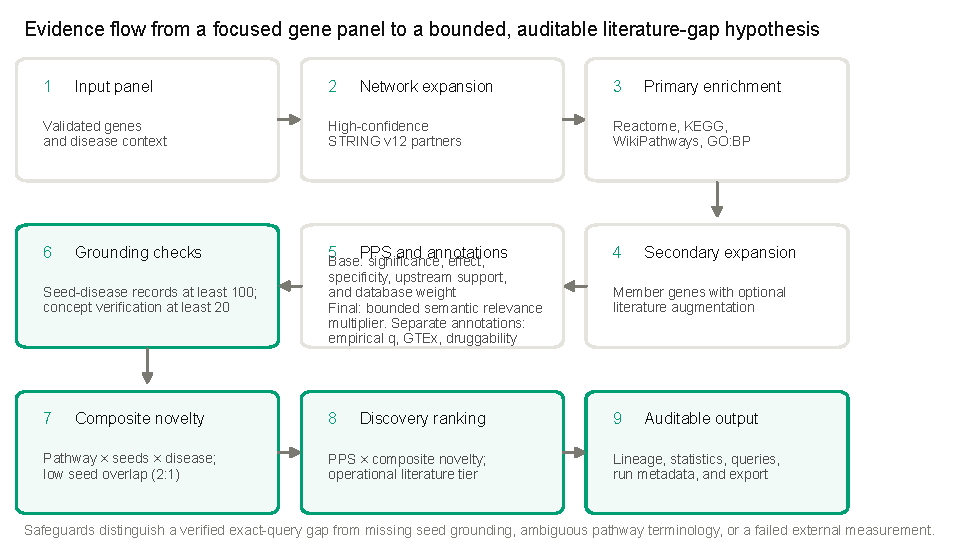
\includegraphics[width=0.98\textwidth]{figures/fig1_cardioxnet_workflow.pdf}
  \caption{CardioXNet evidence flow. A normalized seed panel is expanded through STRING, enriched across complementary pathway resources, and re-expanded from primary-pathway member genes, optionally augmented with literature-derived genes for the highest-priority primaries. Base PPS summarizes statistical and pathway evidence; final PPS adds a bounded semantic cardiovascular-relevance multiplier. Permutation support, GTEx expression, and druggability remain separate annotations. Seed grounding and pathway-concept checks precede the exact-query novelty calculation. The Discovery Score combines final PPS with composite novelty, and the output preserves lineage, component values, query provenance, and run metadata.}
  \label{fig:workflow}
\end{figure*}

\section{Methods}
\label{sec:methods}

\subsection{System Overview and Inputs}
CardioXNet accepts human gene symbols, an optional cardiovascular disease context, and a configurable analysis depth; symbols are normalized and deduplicated before analysis. Figure~\ref{fig:workflow} summarizes the pipeline. Each run is persisted as a structured analysis object, so the application programming interface (API), web interface, comma-separated value export, and report generator all read one result representation.

The benchmark used five seed genes per panel and the balanced preset. The four real panels covered inflammatory remodeling in heart failure, sarcomeric and nuclear-envelope biology in cardiomyopathy, inherited arrhythmia channels, and lipid or endothelial biology in myocardial infarction; the three controls comprised one coherent off-target olfactory-receptor panel and two random protein-coding panels (Table~\ref{tab:panels}).

\begin{table*}[t]
\caption{Regenerated benchmark design and output counts. All analyses used five human seed genes and the balanced configuration.}
\label{tab:panels}
\centering
\small
\begin{tabular}{p{2.15cm}p{1.85cm}p{6.8cm}p{2.7cm}r}
\toprule
Panel & Type & Seed genes & Disease context & Hypotheses \\
\midrule
HF inflammatory & Real & VEGFA, MMP9, IL6, TNF, ACE & Heart failure & 21 \\
DCM structural & Real & MYH7, TTN, LMNA, MYBPC3, TNNT2 & Cardiomyopathy & 34 \\
Arrhythmia channels & Real & SCN5A, KCNQ1, KCNH2, RYR2, CACNA1C & Arrhythmia & 41 \\
MI ischemic & Real & LDLR, APOB, PCSK9, NOS3, EDN1 & Myocardial infarction & 37 \\
Olfactory & Off-target control & OR51E2, OR2W1, OR1A1, OR5K1, OR10A4 & Heart failure & 12 \\
Random 1 & Random control & RPF2, CLRN3, PRKAG1, OR8U9, CACNA1D & Heart failure & 19 \\
Random 2 & Random control & C2CD4A, GORASP1, CHIC1, VCY, PLCD4 & Heart failure & 9 \\
\bottomrule
\end{tabular}
\end{table*}

\subsection{Network and Pathway Expansion}
For each validated seed, CardioXNet retrieves high-confidence human protein associations from STRING v12.0; the union of seeds and neighbors forms the functional neighborhood. Over-representation analysis then runs through g:Profiler against Reactome, KEGG, WikiPathways, and Gene Ontology Biological Process \cite{milacic2024reactome,kanehisa2023kegg,agrawal2024wikipathways,go2023} at a false-discovery-rate threshold of 0.05. Term size, query size, effective domain size, observed overlap, and evidence genes are carried forward so effect size can be computed explicitly.

Primary pathways already annotated to the seed genes are removed so the expansion targets mechanisms that do not trivially restate the input. Primary-pathway member genes are re-enriched to generate secondary pathways, and the highest-priority primaries may first be augmented with literature-derived genes. Redundant pathways are collapsed by evidence-gene overlap, and support from multiple primaries is retained as an upstream-support count.

Cardiovascular relevance $A_j\in[0,1]$ is a deterministic lexical heuristic derived from pathway terminology, optional disease-context terms, and explicit noncardiac penalties; it is not a trained or externally validated classifier. Candidates below $A_j=0.001$ were removed. After reranking, the first 30 candidates were retained without a name condition to preserve vocabulary-divergent hypotheses; positions 31--100 required $A_j\geq0.30$ or an explicit cardiovascular or disease term, and lower positions required $A_j\geq0.50$ up to a 100-candidate cap. The final strict pathway-name gate was disabled because universally requiring a cardiovascular word would be circular for discovery. Semantic terminology therefore influences selection and ranking, but no retained candidate is required to carry a cardiovascular term in its label.

\subsection{Bounded g:Profiler Execution}
The official g:Profiler Python library calls \texttt{requests.post} internally without exposing a request timeout. CardioXNet therefore runs each profile call in a fresh spawned process under a configurable hard wall-clock deadline (120 s by default). The worker writes a complete response to a private temporary file and emits a completion sentinel only after that write succeeds; if the deadline expires, the parent terminates and reaps the worker. Transient failures receive bounded retries with exponential backoff (two by default), and exhaustion raises an explicit pipeline error. An interrupted, unreadable, malformed, or partial response is never treated as enrichment data, whereas a complete empty response is a valid result indicating no enriched terms.

\subsection{Pathway Prioritization Score}
The PPS replaces an earlier significance-times-gene-count formula that favored generic, large gene sets. The base score for pathway $j$ is
\begin{equation}
 B_j=w_{d,j}\left(0.30S_j+0.30E_j+0.25G_j+0.15R_j\right),
\end{equation}
and the score used for downstream ranking is
\begin{equation}
\mathrm{PPS}_j=B_j(1+A_j),
\label{eq:pps}
\end{equation}
where $w_{d,j}$ is a source-specific database weight and $A_j$ is the semantic cardiovascular-relevance value defined above. Network topology is reported separately and does not enter PPS: one-hop proximity is not used as a multiplier because the evidence genes were selected from that same functional neighborhood, so rewarding the overlap again would reuse rather than corroborate the enrichment evidence. PageRank is computed later for topology interpretation. The multiplier $1+A_j$ is bounded in $[1,2]$, and both it and $A_j$ are retained in the score breakdown. The four normalized base-score terms are
\begin{align}
S_j &= \min\left(\frac{-\log_{10}(p_{\mathrm{adj},j})}{10},1\right),\\
E_j &= \min\left(\frac{\log_2(F_j)}{\log_2(10)},1\right),\\
G_j &= 1-\min\left(\frac{\log_{10}(T_j)}{\log_{10}(500)},1\right),\\
R_j &= \min\left(\frac{C_j}{5},1\right).
\end{align}
Here, $F_j$ is fold enrichment, $T_j$ is annotated term size, and $C_j$ is the number of primary pathways supporting the candidate. Statistical significance saturates at $p_{\mathrm{adj}}=10^{-10}$, and fold enrichment saturates at 10-fold, limiting the influence of numerical floors and annotation scale. A twofold minimum enrichment is applied when the required universe sizes are available.

\subsection{Literature Saturation, Grounding, and Discovery Score}
The literature query is constructed as a strict conjunction of three title/abstract clauses: the pathway concept, contributing seed genes, and disease context. CardioXNet retrieves a limited set of abstracts for evidence display but separately obtains the uncapped PubMed record count $H_j$ returned by that query. Literature saturation is
\begin{equation}
L_j=\min\left(\frac{\log_{10}(H_j+1)}{\log_{10}(1001)},1\right),
\end{equation}
and literature novelty is $1-L_j$. The gene novelty component is based on the fraction of pathway evidence genes not present in the seed panel. These terms are combined at a 2:1 literature-to-gene ratio to produce $N_j$. The primary ranking metric is
\begin{equation}
D_j=\mathrm{PPS}_jN_j.
\label{eq:discovery}
\end{equation}

Two safeguards constrain interpretation. First, the seed genes must return at least 100 PubMed records in the specified disease before pathway-level novelty is grounded; panels below this threshold receive the categorical state \emph{Ungrounded} and are not placed on the same novelty scale. Second, an empty pathway intersection counts as a verified gap only when the pathway concept itself has at least 20 records; otherwise it is flagged unverified and assigned a conservative proxy corpus rather than maximal novelty. A failed count request is recorded as not measured and can never become a zero.

The terms Highly Novel, Novel, Emerging, and Established are operational tiers for the composite novelty value, not claims of biological originality. In the main text, ``zero records'' always means that no PubMed title/abstract record matched the prespecified query in the corresponding retrieval snapshot. It does not mean that related biology is absent under other terminology or in full text.

\subsection{Permutation, Tissue, and Druggability Evidence}
Each pathway overlap is tested against 1,000 size-matched random neighborhoods. The baseline is a pinned snapshot of 19,410 human protein-coding symbols; analysis genes absent from that snapshot are added so the observed set is drawable from the null. Effective run-specific pools therefore contained 19,410 to 19,415 genes. The empirical value is calculated with the finite-sampling correction \cite{phipson2010permutation}:
\begin{equation}
p_{\mathrm{emp}}=\frac{1+\sum_{b=1}^{B}I(O_b\ge O_{\mathrm{obs}})}{B+1},
\end{equation}
where $B=1000$. The resolution floor is therefore $1/1001\approx 9.99\times10^{-4}$. Benjamini-Hochberg correction is applied across all testable reported pathways \cite{benjamini1995fdr}. Untestable pathways retain null values and are excluded from the correction family rather than assigned $p=1$. The null tests whether overlap exceeds a random gene-set expectation and does not rank already strong candidates; Section~\ref{sec:discussion} states its degree limitation.

Cardiac expression is evaluated against GTEx v8 left-ventricular and atrial-appendage data \cite{gtex2020atlas}. Druggability starts from an embedded curated snapshot derived from DrugBank v5.1.10, TTD 2023, ChEMBL v31, and related references, optionally adding live Open Targets evidence \cite{ochoa2021opentargets,zdrazil2024chembl}. Both annotate ranked hypotheses but enter neither PPS nor the Discovery Score. Open Targets completion and failure counts are persisted, so an incomplete lookup cannot be presented as a verified zero.

\subsection{Reproducibility and Software Verification}
The permutation background, sorted sampling universe, private random-number generator, and default seed (20260821) are pinned. External resources remain live and can drift, so each result records retrieval timestamps, endpoints, configured resource identifiers, and whether identifiers were verified from a live response.

Every external client distinguishes a failed request from a measured zero, since the two are otherwise indistinguishable in a saturation metric. A silent Open Targets schema change had made all external druggability lookups fail while reporting zero targets; the repaired query returns explicit evidence and records failures as unavailable. GTEx lookup no longer substitutes an approximate gene when an exact symbol is absent, and STRING parsing skips and reports malformed records rather than discarding a whole response. Regression tests cover scoring, multiple testing, grounding, these sentinels, g:Profiler deadlines, persistence, and exports; browser-level checks cover ranking order, missing-value rendering, evidence breakdowns, table integrity, navigation, and downloads against a committed deterministic fixture.

The user interface separates setup, ranked comparison, and pathway audit. Figures~\ref{fig:ui-results} and~\ref{fig:ui-audit} show the two principal application evidence views. The compact table supports comparison without hiding definitions, and the detail page presents the exact literature count beside the discovery lineage. Exported data retain the underlying component values.

\section{Benchmark Design}
\label{sec:benchmark}

\subsection{Regenerated Benchmark}
All benchmark analyses were regenerated after corrections that affected filtering, query construction, and seeded permutation sampling because carrying forward previous values would have mixed incompatible candidate sets. The regenerated runs used STRING v12.0, the configured g:Profiler identifier \texttt{e104\_eg51\_p15}, GTEx v8, an embedded curated drug-target snapshot with optional Open Targets evidence, and PubMed. The g:Profiler identifier is declared configuration metadata rather than a build value verified from the response. The four real panels produced 133 hypotheses and the three controls produced 40.

The benchmark tests four questions. First, is the PPS ranking behavior consistent with its specificity-aware design? Second, do uncapped exact-query counts discriminate among hypotheses better than the number of abstracts retrieved? Third, does the grounding rule preserve the intended real-panel and control invariants after regeneration? Fourth, is novelty measured at the end of 2020 associated with subsequent publication activity?

\subsection{Temporal Holdout}
The temporal holdout included all 133 real-panel hypotheses. Literature was censored at December 31, 2020, and records from January 1, 2021 through the follow-up snapshot were counted separately. Composite novelty, operational tier, grounding, and Discovery Score were recomputed from pre-cutoff measurements under the same rules. Eleven hypotheses met the verified-gap rule at the cutoff and none was Ungrounded. Relative growth was $H_{\mathrm{post}}/(H_{\mathrm{pre}}+1)$, compared with cutoff scores by Spearman rank correlation; a sensitivity analysis excluded the 11 intersections with zero pre-cutoff records. Pathways overlap within panels, so these correlations are descriptive and $n$ denotes hypotheses rather than independent biological replicates.

\section{Results}
\label{sec:results}

\subsection{PPS Ranking Was Consistent With Its Specificity-Aware Design}
The previous score multiplied statistical significance by raw evidence-gene count and so structurally favored larger annotations. In the regenerated heart-failure benchmark the highest final-PPS pathway contained six annotated genes, and the 15 highest-PPS pathways spanned 5 to 103 genes, with term size inversely rank-associated with final PPS (Spearman $\rho=-0.9293$; Fig.~\ref{fig:specificity}). Gene-set specificity is an explicit PPS component, so this is a consistency check rather than independent validation or a paired comparison with the previous score.

\begin{figure*}[t]
  \centering
  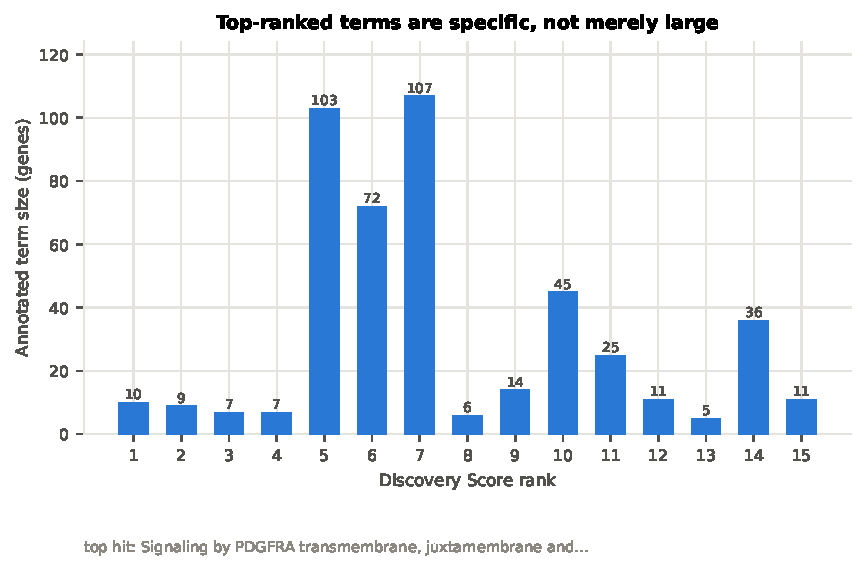
\includegraphics[width=0.94\textwidth]{figures/fig2_term_specificity.pdf}
  \caption{Annotated term size versus final PPS for the 15 highest-PPS heart-failure hypotheses ($n=15$); numeric labels give final-PPS rank. Gene-set specificity is an explicit score component, so this is a consistency check, not independent validation.}
  \label{fig:specificity}
\end{figure*}

\subsection{Seven Cardiovascular Intersections Met the Verified-Gap Rule}
Seven of 133 real-panel hypotheses met the prespecified verified-gap rule: a grounded seed-disease panel, a searchable pathway concept, and zero records for the exact title/abstract query (Table~\ref{tab:candidates}, Fig.~\ref{fig:gaps}). In structural cardiomyopathy, GAB1 signalosome and NTRK2 signaling returned zero records at 15.8-fold and 17.5-fold enrichment, with evidence genes SRC, EGFR, EGF and SRC, CDK5, CDK5R1 respectively. In arrhythmia, cGMP-PKG and GPER1 signaling returned zero records at 7.9-fold and 8.4-fold. In the ischemic panel, P2Y12, GPER1, and oxytocin signaling met the rule, while inflammasomes returned one record.

These are panel-level literature gaps, not claims about a pathway in isolation. For P2Y12, CardioXNet asks whether that pathway has been reported jointly with the contributing genes of the LDLR, APOB, PCSK9, NOS3, and EDN1 panel in the specified myocardial-infarction context; the zero identifies an unreported intersection between defined domains rather than an unknown pathway. Each candidate remains a computational hypothesis requiring synonym-expanded review and experimental assessment.

\begin{table*}[t]
\caption{Representative cardiovascular hypotheses from the regenerated benchmark. ``Exact-query records'' is the uncapped count of PubMed title/abstract records matching the prespecified pathway, contributing-gene, and disease query in the benchmark snapshot. The empirical $q$-value is Benjamini-Hochberg adjusted under the uniform genome-scale permutation null. Zero denotes the operational verified-gap state, not absence of related biology under all terminology.}
\label{tab:candidates}
\centering
\scriptsize
\setlength{\tabcolsep}{3pt}
\begin{tabular}{p{1.75cm}p{4.65cm}rrrrp{3.05cm}}
\toprule
Panel & Pathway candidate & Discovery & Fold & Empirical $q$ & Exact-query records & Interpretation \\
\midrule
DCM structural & GAB1 signalosome & 2.009 & 15.8 & 0.00162 & 0 & Growth-factor adaptor bridge \\
DCM structural & NTRK2 (TRKB) signaling & 1.984 & 17.5 & 0.00162 & 0 & Neurotrophin-signaling bridge \\
Arrhythmia channels & cGMP-PKG signaling & 1.907 & 7.9 & 0.00124 & 0 & Cyclic-nucleotide regulation \\
Arrhythmia channels & GPER1 signaling & 1.865 & 8.4 & 0.00124 & 0 & Hormone-responsive signaling \\
MI ischemic & P2Y12 signaling & 1.808 & 8.1 & 0.00127 & 0 & Platelet signaling linked to seed panel \\
MI ischemic & GPER1 signaling & 1.800 & 6.7 & 0.00127 & 0 & Shared vascular-signaling candidate \\
MI ischemic & Oxytocin signaling & 1.749 & 7.0 & 0.00127 & 0 & Hormone-responsive signaling candidate \\
HF inflammatory & MET activates PTK2 signaling & 1.098 & 21.0 & 0.00105 & 92 & Less sparse but high-effect remodeling candidate \\
\bottomrule
\end{tabular}
\end{table*}

\subsection{Uncapped Exact-Query Counts Preserved Discrimination}
For the heart-failure panel, uncapped exact-query counts spanned 31 to 10,868 records (350.6-fold), whereas retrieved abstracts varied only from 26 to 30 because retrieval is capped. Figure~\ref{fig:saturation} shows why the query count and the displayed evidence set are not interchangeable: deriving saturation from retrieved items compresses a 350.6-fold range into 1.15-fold, removing most of the signal.

\begin{figure*}[t]
  \centering
  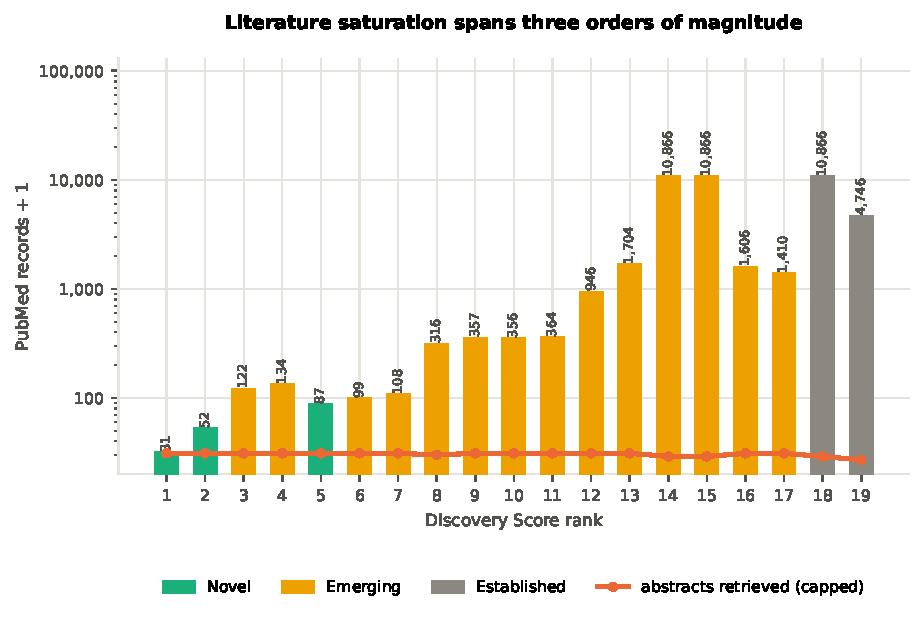
\includegraphics[width=0.94\textwidth]{figures/fig3_literature_saturation.pdf}
  \caption{Exact-query literature counts for the 20 highest-ranked heart-failure hypotheses. Bars show the uncapped PubMed title/abstract count plus one on a logarithmic scale, hatched by operational literature tier; the diamond-marked line shows the capped display set plus one. Labels give untransformed query counts.}
  \label{fig:saturation}
\end{figure*}

\subsection{Grounding Separated Real Panels From Controls}
The real-panel seed-disease corpora held 10,868, 2,487, 1,538, and 2,373 records, all at least 15 times the grounding threshold; the control corpora held 0, 6, and 1. All 40 control hypotheses were Ungrounded and none of the 133 real-panel hypotheses was. Both invariants held exactly after regeneration (Fig.~\ref{fig:controls}).

This test addresses a specific failure mode. Before grounding, off-target and random panels produced more Highly Novel calls than the cardiovascular panels, because every empty intersection received maximal novelty. The corrected system treats insufficient seed literature as undefined novelty rather than strong evidence. Since this failure motivated the gate and the same panels were retained for regression testing, the 40/40 versus 0/133 separation is a correctness invariant, not an unbiased specificity estimate.

\begin{figure*}[t]
  \centering
  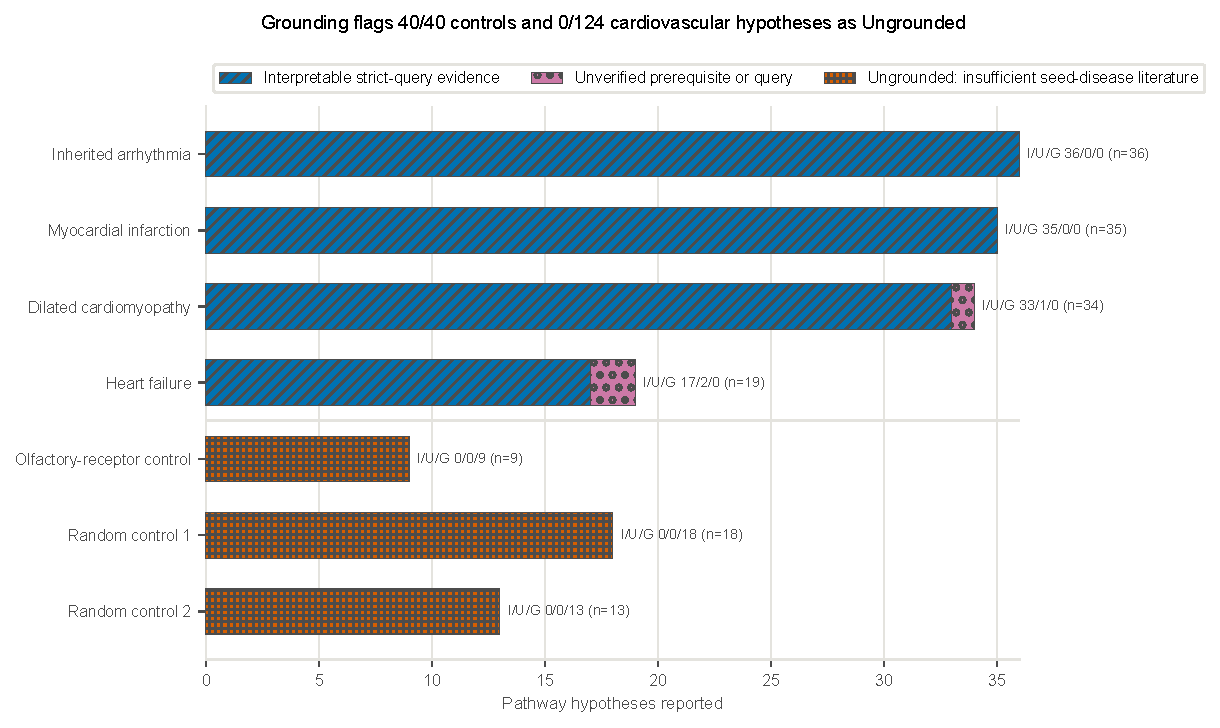
\includegraphics[width=0.94\textwidth]{figures/fig5_negative_controls.pdf}
  \caption{Grounding regression benchmark. Diagonal hatching denotes an interpretable literature tier; cross-hatching denotes Ungrounded hypotheses whose seed panels had insufficient disease literature. Labels give grounded over total hypotheses. These development-set invariants test implementation behavior and do not estimate out-of-sample specificity.}
  \label{fig:controls}
\end{figure*}

\subsection{Temporal Holdout Showed Negligible Overall Association}
Across all 133 hypotheses, the Discovery Score at the 2020 cutoff showed negligible rank association with publication growth in the follow-up retrieval snapshot ($\rho=-0.0635$). Composite novelty alone was similarly near zero ($\rho=-0.0283$), and PPS alone was weakly negative ($\rho=-0.1462$). Among the 122 hypotheses with nonzero pre-cutoff counts, the Discovery Score association remained near zero ($\rho=0.0225$).

Within-panel values were heterogeneous ($\rho=0.7165$ heart failure, $0.0485$ arrhythmia, $-0.2235$ structural cardiomyopathy, $-0.3826$ myocardial infarction) and four descriptive panel results do not support a general forecasting claim. At the cutoff, the Highly Novel, Novel, Emerging, and Established tiers held 18, 55, 48, and 12 hypotheses with median growth 0, 0.6970, 0.6061, and 0.5413. Figure~\ref{fig:holdout} therefore bounds the Discovery Score as a triage measure: sparse intersections are not necessarily where publication activity will increase.

\begin{figure*}[t]
  \centering
  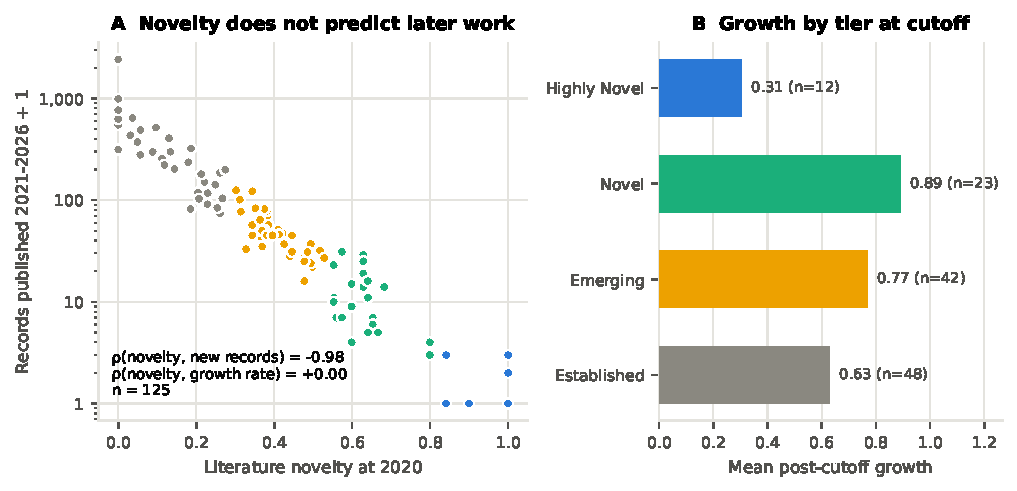
\includegraphics[width=0.96\textwidth]{figures/fig4_temporal_holdout.pdf}
  \caption{Temporal holdout using all 133 real-panel hypotheses, with literature censored at December 31, 2020 and follow-up records counted in a separate snapshot. (A) Discovery Score versus post-cutoff growth ($\rho=-0.0635$); the measurable-only sensitivity result was $\rho=0.0225$ ($n=122$). (B) Growth stratified by operational tier at the cutoff: boxes span the interquartile range, center lines are medians, whiskers extend to 1.5$\times$ IQR, points are outliers, and diamonds are means. Pathways overlap within panels, so correlations are descriptive and do not establish predictive validity.}
  \label{fig:holdout}
\end{figure*}

\begin{figure*}[t]
  \centering
  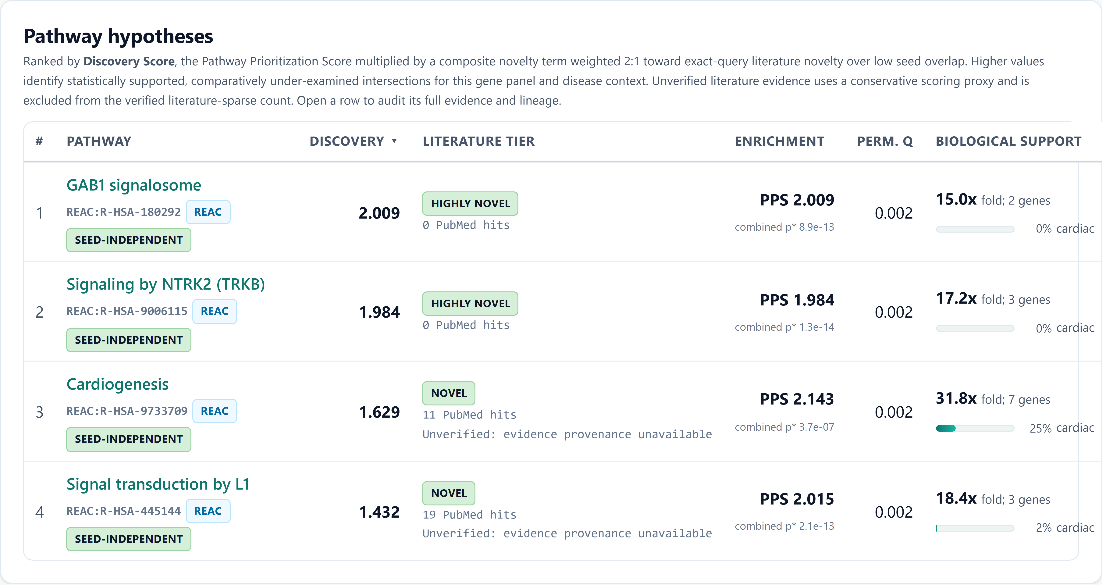
\includegraphics[width=0.96\textwidth]{figures/fig6a_application_ranked_results.pdf}
  \caption{Ranked-results application view, comparing Discovery Score, operational literature tier and evidence status, PPS, empirical $q$-value, fold enrichment, and cardiovascular relevance without collapsing them into one metric. This cropped deterministic cardiomyopathy fixture demonstrates interface behavior only.}
  \label{fig:ui-results}
\end{figure*}

\begin{figure*}[t]
  \centering
  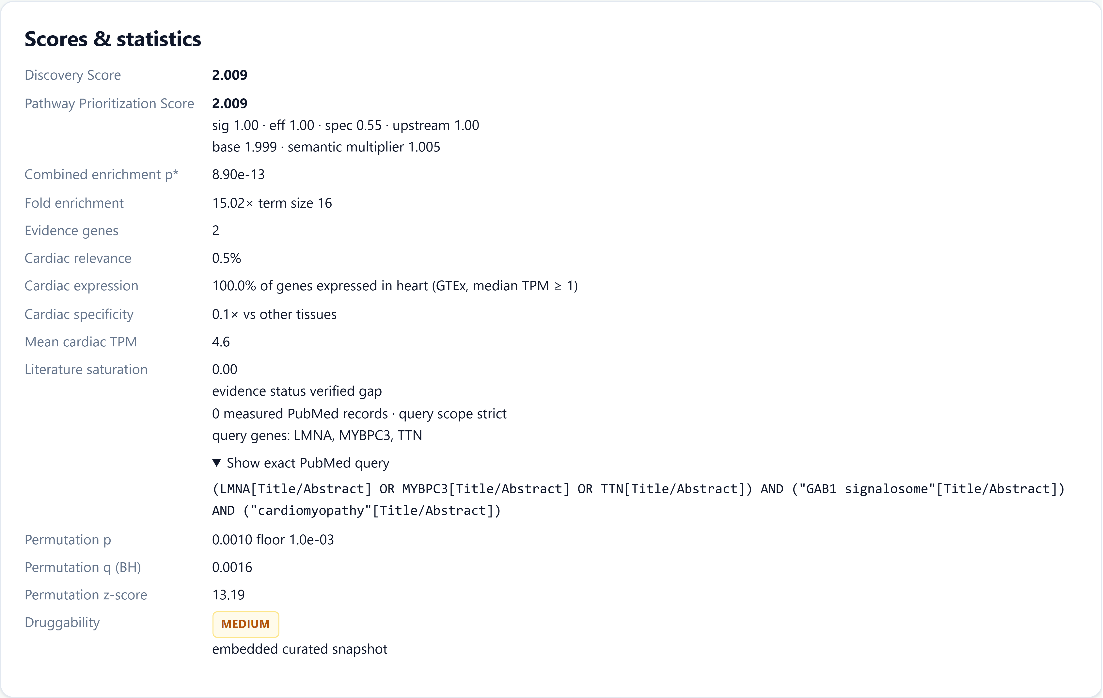
\includegraphics[width=0.94\textwidth]{figures/fig6b_application_pathway_audit.pdf}
  \caption{Pathway-audit application view. The score card exposes the measured PubMed record count, query scope and exact query, scoring components, enrichment and permutation statistics, cardiac expression, and druggability provenance. The deterministic fixture demonstrates inspectability only.}
  \label{fig:ui-audit}
\end{figure*}

\begin{figure*}[t]
  \centering
  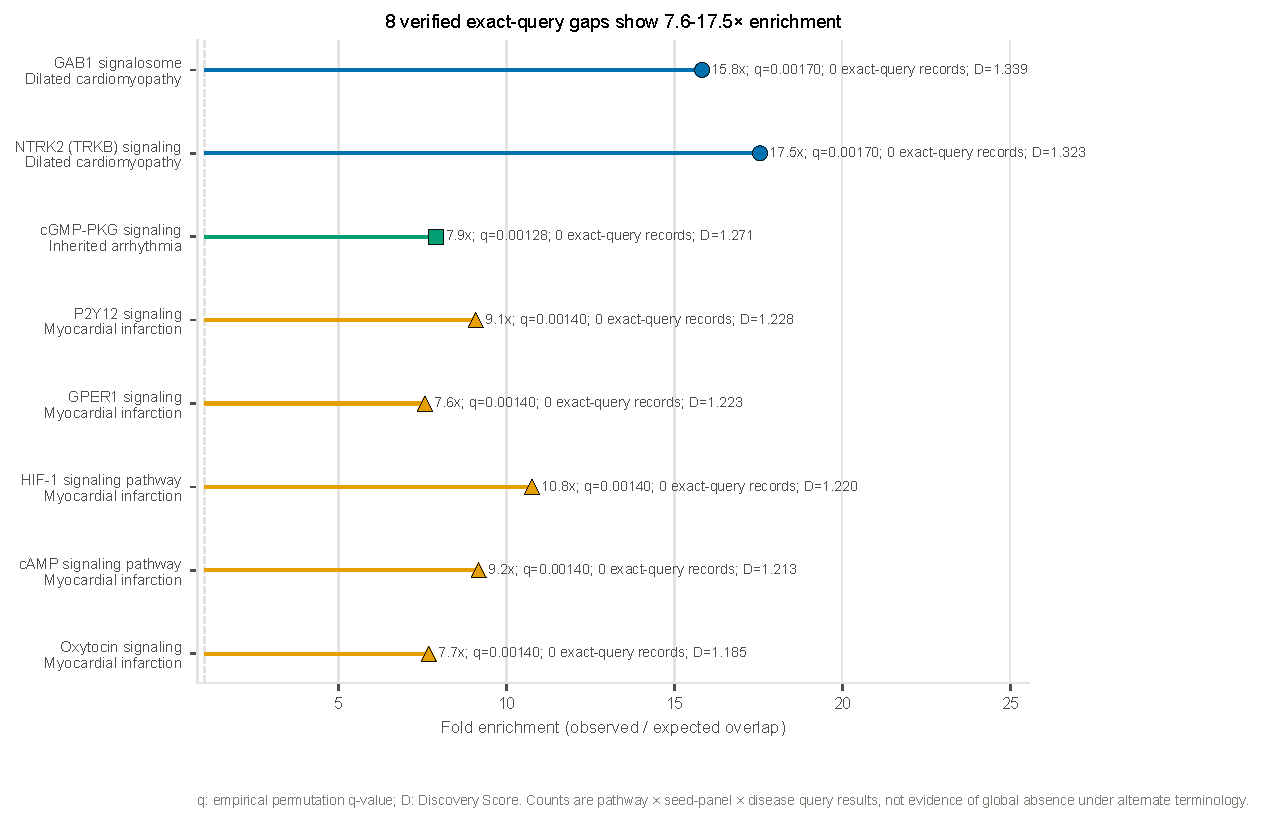
\includegraphics[width=0.98\textwidth]{figures/fig7_cardiovascular_discovery_gaps.pdf}
  \caption{The seven cardiovascular hypotheses meeting the verified exact-query gap rule. Horizontal position gives fold enrichment; labels report the empirical $q$-value, exact-query record count, and Discovery Score ($D$). Color and marker shape redundantly encode disease panel. Counts are specific to the prespecified query in the benchmark snapshot and do not establish global biological novelty.}
  \label{fig:gaps}
\end{figure*}

\subsection{Live-Resource Variation Propagates Through Filtering}
One paired back-to-back comparison returned identical functional neighborhoods (219 genes, 2,261 STRING interactions) and identical primary enrichment (1,787 pathways), but differed by one secondary pathway (3,045 versus 3,046). The redundancy filter amplified this into 34 versus 37 final pathways. Among the 33 shared pathways, six PPS values changed, the largest relative difference was 6.0 percent, and no literature tier changed. A single pair does not estimate a noise distribution; it shows that live-resource variation propagates through redundancy filtering, so reported scores require run dates and apparent differences require repeated analysis.

\section{Discussion}
\label{sec:discussion}

\subsection{Novelty and Practical Meaning}
CardioXNet's main contribution is separating three concepts that are often conflated: evidence-weighted cardiovascular prioritization, literature saturation, and whether a novelty estimate is interpretable at all. PPS asks whether a pathway has statistical, annotation-specific, upstream, source, and lexical cardiovascular support. Literature saturation asks how much has been indexed at one defined intersection. Grounding asks whether a low count can be interpreted at all. Keeping literature saturation and grounding separate from pathway support makes a zero auditable and prevents an irrelevant panel from appearing more innovative than a well-grounded cardiovascular panel.

The benchmark nominates several cardiovascular connections for manual review. GAB1 and NTRK2 signaling in the structural cardiomyopathy panel suggest growth-factor-adaptor and neurotrophin routes linking sarcomeric or nuclear-envelope seeds to downstream signaling genes; cGMP-PKG and GPER1 in the arrhythmia panel suggest modulation beyond the input ion channels; P2Y12 and GPER1 in the ischemic panel connect platelet and hormone-responsive signaling with lipid and endothelial seeds. These are testable pathway-level hypotheses from enrichment evidence and a prespecified exact-query gap, not verified mechanisms, causal claims, or guarantees of clinical relevance.

The temporal holdout marks this boundary rather than validating a forecast. The overall association with later growth was negligible and panel-specific associations varied in direction. Low saturation can indicate a productive opportunity, a vocabulary mismatch, a deliberately narrow intersection, or an unproductive question, so expert review and experimental validation remain necessary. The defensible use is to reduce a large enrichment output to a transparent shortlist for mechanistic evaluation.

\subsection{Comparison With Conventional Enrichment Workflows}
Conventional enrichment tools identify overrepresented annotations correctly but do not generally treat literature opportunity as a separate, validity-gated measurement. CardioXNet does not replace g:Profiler or the underlying curated resources; it adds network expansion, specificity-aware ranking, uncapped exact-query literature counts, seed grounding, and a unified audit interface. It is intended for small, well-supported starting panels when the goal is to reason outward toward connections not already explicit in the input.

The design also avoids a common presentation failure: describing a composite score as a normalized enrichment score. PPS is not gene set enrichment analysis and contains no running-sum statistic or permutation normalization. Its components, saturation points, and multipliers are reported directly. The empirical permutation $q$-value is separate from PPS and answers a narrower question about overlap relative to a random genome-scale neighborhood.

\subsection{Limitations}
Literature novelty is lexical, field-restricted, and database-dependent. Identifiers and uncommon pathway nomenclature may be poorly represented in PubMed even when the mechanism is well studied; the pathway-concept check reduces but cannot eliminate this risk. Exact title/abstract queries are deliberately narrow and do not search full text, so any zero requires synonym expansion and expert review.

The permutation null samples uniformly from a protein-coding background and does not preserve STRING degree, so it supports comparison with a random gene-set expectation but may be anti-conservative for highly connected neighborhoods; a degree-aware null would require a pinned genome-wide interaction-degree reference. Four real panels and three controls are not comprehensive biological validation across cardiovascular phenotypes, and because the controls informed development of the grounding gate, their complete separation cannot estimate out-of-sample specificity.

Live resources drift. STRING, g:Profiler, GTEx endpoints, Open Targets, and PubMed can change in content or schema, so the full pipeline is not bit-reproducible even when its random components are pinned; each run must retain retrieval timestamps, endpoints, and configured or response-verified resource identifiers. The paired rerun reported in Section~\ref{sec:results} is a single observation, not an estimated noise floor.

The temporal analysis is likewise descriptive. Pathways overlap within panels and therefore are not independent biological replicates. Four panels are insufficient to characterize cross-phenotype heterogeneity, and publication growth measures scientific attention rather than biological truth.

Finally, GTEx expression is bulk-tissue context rather than cell-type or disease-state evidence, druggability indicates targetability rather than therapeutic benefit, and semantic cardiovascular relevance can miss mechanisms described with distant vocabulary. Every CardioXNet output remains a hypothesis for independent validation.

\section{Conclusion}
CardioXNet provides an auditable path from a focused cardiovascular gene panel to statistically supported, literature-sparse query intersections. Its specificity-aware PPS reduces generic-term dominance, uncapped PubMed counts preserve a 350.6-fold literature range that capped retrieval compresses to 1.15-fold, and the grounding gate maintains the 0/133 real-panel and 40/40 control invariants. Seven hypotheses met the verified exact-query gap rule, while the all-hypothesis temporal holdout showed negligible association with later publication growth ($\rho=-0.0635$). CardioXNet is therefore suited to prioritizing under-examined cardiovascular connections for expert review and experiment, with query provenance, evidence components, and validity boundaries kept visible.

\section*{Data and Code Availability}
The manuscript workspace includes the benchmark manifest, generation scripts, vector and 600 dpi raster figures, structured tables, and a deterministic application fixture. Each analysis is stored as machine-readable JSON with ranked results exported as CSV. Live resources should be re-queried with the run date recorded; the pinned 19,410-symbol baseline, run-specific background augmentation, and random seed preserve the permutation design.

\bibliographystyle{IEEEtran}
\bibliography{references}
\EOD

\end{document}
